% Template for ICASSP-2024 paper; to be used with:
%          spconf.sty  - ICASSP/ICIP LaTeX style file, and
%          IEEEbib.bst - IEEE bibliography style file.
% --------------------------------------------------------------------------
\documentclass{article}
\usepackage{spconf,amsmath,graphicx}
\usepackage{multirow}              % per-host recipe table
\usepackage{microtype}             % kills sub-3pt overfull, polishes justification
\usepackage{csquotes}
\usepackage{comment}
\usepackage{xcolor}

% Example definitions.
% --------------------
\def\x{{\mathbf x}}
\def\L{{\cal L}}

% Title.
% ------
\title{Referring Multi-Object Tracking in Moving-Camera Videos via Global Motion Compensation}
%
% Single address.
% ---------------
\name{Author(s) Name(s)}
\address{Author Affiliation(s)}
%
\begin{document}
\ninept
%
\maketitle
%
\begin{abstract}
  Referring multi-object tracking (RMOT) takes a video and a language expression as input and tracks all referred objects. Many tracking requirements involve how an object moves rather than how it appears. However, in a video captured by a moving camera, a parked vehicle may appear to move, while a moving vehicle may show little displacement. Existing RMOT methods relate motion with text but do not explicitly remove camera-induced motion. In this paper, we propose extracting residual motion across frames by estimating camera motion in driver-view videos and compare motion characteristics with the query expression. We consider the motion-matching extent and integrate it with the RMOT method's prediction result through late fusion. In the evaluation, we verify the performance gain of taking the motion compensation module as a plug-in across different RMOT hosts.
\end{abstract}
%
\begin{keywords}
  referring multi-object tracking, motion compensation, motion-language alignment
\end{keywords}

%-------------------------------

\section{Introduction}
\label{sec:intro}
Referring multi-object tracking (RMOT) outputs tracking results of the objects described by a free-form language expression. For example, a \enquote{left-vehicles-in-red} description targets the red vehicles on the left. However, many descriptions focus on moving objects, such as \enquote{moving cars} or \enquote{a vehicle turning left}. In videos captured by a moving camera, the observed motion is a mixture of object motion and camera motion; thus, a static car may appear to move, while a moving car may appear static across frames.

Previous RMOT methods~\cite{transrmot,ikun,flexhook} match language expressions to objects. VMRMOT~\cite{vmrmot} considers explicit motion cues, such as changes in direction and speed, in the matching process. These methods compute motion from the object's bounding-box displacement across frames, which mixes object motion with camera motion. On the other hand, conventional multi-object tracking (MOT) methods propose to remove camera motion. BoT-SORT~\cite{botsort} estimates camera-induced image motion, while UCMCTrack~\cite{ucmctrack} stabilizes object trajectories. Overall, how motion compensation can be extended to RMOT is still underexplored.

In this paper, we propose separating object motion from camera motion and providing motion cues for RMOT methods. It consists of four stages. First, the geometric transformation across frames is estimated to measure camera motion. The estimated transformations are accumulated across frames to reliably measure object motion. Second, residual velocity, which represents object motion after removing camera motion, is computed across frames and used as a temporal motion feature. Third, a Contrastive Motion Aligner is developed to compare motion features with language expressions and produce a motion-matching score. Finally, the motion-matching score is scaled by a host-specific weight and added to the host's matching score. Here, the host model refers to a two-stage RMOT method used as a baseline, such as iKUN~\cite{ikun} and FlexHook~\cite{flexhook}. The proposed process is implemented as a plug-in module, thereby improving existing RMOT baselines without retraining them.

This work connects motion compensation with motion-language modeling for RMOT. Our main contributions are as follows.
\begin{itemize}
  \item We propose a plug-in module that aligns the object's residual velocity with the referring expression, thereby improving the host RMOT method without modifying or retraining it.
  \item Across two host RMOT methods, i.e., iKUN and FlexHook, the proposed module improves pooled HOTA in all settings. On iKUN, it raises moving-class HOTA from $27.697$ to $37.139\pm0.923$ (approximately $+9.44$ points).
\end{itemize}

%---------------------

\begin{figure*}
  \centering
  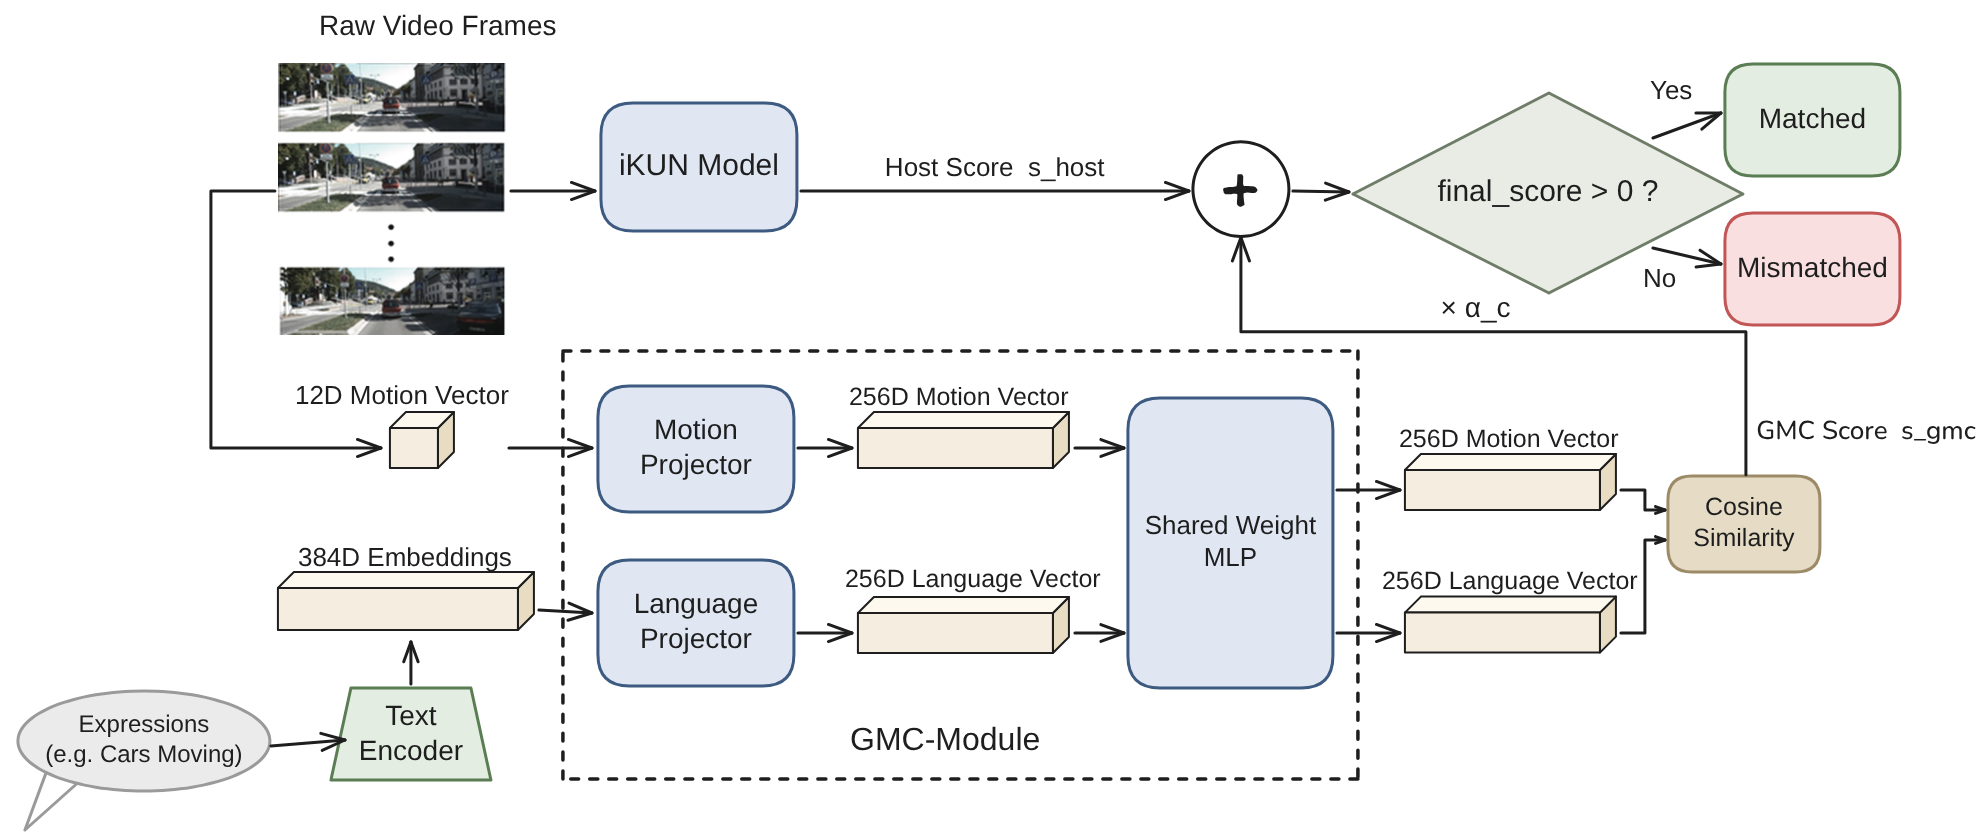
\includegraphics[width=12cm]{figures/Architecture.png}
  \caption{The proposed RMOT framework with the global motion compensation module. The host model (iKUN in this case) predicts an object-language matching score. The GMC module provides an extra matching score to adjust matching results.}
  \label{fig:architecture}
\end{figure*}

\section{Related Works}
\label{sec:related}
\subsection{Referring Multi-Object Tracking}
TransRMOT~\cite{transrmot} introduced the RMOT task on the Refer-KITTI dataset. Later methods improved different parts of this task. iKUN~\cite{ikun} separated language-based object matching from object tracking, while FlexHook~\cite{flexhook} improved how visual and language information interact. ReferGPT~\cite{refergpt} used a multimodal large language model to describe existing object tracks, and MEX~\cite{mex} provided a memory-efficient module for matching tracks with language.

Recent RMOT methods~\cite{deeprmot} further improve models' understanding of object descriptions. STORM~\cite{storm} unifies grounding and tracking in an end-to-end multimodal large language model. VMRMOT~\cite{vmrmot} explicitly represents motion using information such as position, direction, changes in distance, and changes in speed. These methods estimate object motion from the object's bounding-box movements across frames.

\subsection{Motion Compensation in Tracking}
Camera motion compensation is widely used in traditional multi-object tracking. BoT-SORT~\cite{botsort} estimates camera-induced motion across frames. UCMCTrack~\cite{ucmctrack} estimates how the camera moves relative to the road. EMAP~\cite{emap} further separates the camera's turning and movement from object motion within the Kalman prediction process.

These methods demonstrate that compensating for camera motion can improve tracking. However, how to integrate compensated motion cues with language expressions to improve RMOT remains underexplored.

%------------------------------------


\section{Method}
\label{sec:method}
Figure~\ref{fig:architecture} shows the proposed RMOT framework with the global motion compensation (GMC) module. The GMC module is attached to a two-stage RMOT method, iKUN~\cite{ikun} in this case. iKUN performs object detection and tracking and then outputs object-language matching scores. The inputs to the GMC module are the sequence of object bounding boxes across frames, the video frames, and the language expression. Based on these inputs, it estimates camera motion, extracts residual object motion, aligns it with the language expression, and produces another matching score. The score is then combined with the host model's predicted score to determine the final tracking result. The GMC module consists of four stages: motion compensation, multi-scale residual velocity extraction, motion-language alignment, and late fusion.


\subsection{Motion Compensation}
\label{sec:ego}
As in previous RMOT works, we take Refer-KITTI~\cite{transrmot} as the evaluation benchmark. Refer-KITTI is recorded from a driver-view camera, so the road surface is visible in most frames and stays close to a single plane. For a forward-facing camera the horizon lies near the vertical image center, so the lower half of the frame contains the road surface. We extract Shi-Tomasi keypoints~\cite{shitomasi} in this lower half, excluding the interiors of the tracked object boxes, and track them into the next frame with pyramidal Lucas-Kanade optical flow~\cite{lucaskanade}. The RANSAC~\cite{ransac} algorithm is then employed to estimate the frame-to-frame homography $H_{t-1 \to t}$ that describes the correspondences between keypoints in two frames.

To describe camera motion across more frames, the estimated homographies are accumulated as
\begin{equation}
  H_{t-k \to t} = H_{t-1 \to t} \times H_{t-2 \to t-1} \times \cdots \times H_{t-k \to t-k+1},
  \label{eq:cumulative}
\end{equation}
where $H_{t-k \to t}$ represents the accumulated camera transformation from frame $I_{t-k}$ to frame $I_t$. Instead of repeatedly transforming already-warped coordinates, the accumulated homography is applied only once to the detected objects' centroids. This reduces numerical drift and provides a stable reference for estimating the residual velocity in the next stage.

\subsection{Multi-Scale Residual Velocity}
\label{sec:residual}
Before going into more details, we define the following three velocities:
\begin{itemize}
  \item \textbf{Raw velocity}: Raw velocity is the observed image-plane velocity of an object, computed from the displacement of its centroid between two frames separated by $g$ frames and normalized by the corresponding time interval.
  \item \textbf{Ego-motion-induced velocity}: Ego-motion-induced velocity is the image-plane velocity caused by camera motion, computed from the displacement of the object's location predicted by the homography between two frames separated by $g$ frames and normalized by the corresponding time interval.
  \item \textbf{Residual velocity}: Residual velocity is the camera-motion-compensated object velocity obtained by subtracting the ego-motion-induced velocity from the raw velocity.
\end{itemize}

Based on the accumulated homography matrix and the objects' bounding boxes, we aim to estimate the \textit{residual velocity}. For a temporal gap $g$, the raw velocity $v^{\mathrm{raw}}_{g}$ is calculated by dividing the displacement of the object centroid between two frames ($I_{t-g}$ and $I_{t}$) by the time gap $g$. The raw velocity is mixed with the object's motion and the camera's motion. To remove the camera motion, the accumulated homography is applied to an object's centroid $\boldsymbol{o}_{t-g}$, yielding $\hat{\boldsymbol{o}}_{t}$ that is the predicted centroid at $I_{t}$ under the assumption that the object is static. Then the ego-motion-induced displacement $\hat{\boldsymbol{o}}_{t}-\boldsymbol{o}_{t-g}$ is normalized by the time interval $g$ to estimate the ego-motion-induced velocity $v^{\mathrm{ego}}_{g}$. The residual velocity $v^{\mathrm{res}}_{g}$ is then computed as
\begin{equation}
  v^{\mathrm{res}}_{g} = v^{\mathrm{raw}}_{g} - v^{\mathrm{ego}}_{g}.
  \label{eq:residual}
\end{equation}
This value approximates the motion that a static camera would observe. For example, a parked vehicle has near-zero residual velocity even when camera motion causes a large image displacement. All displacements are normalized by the image dimensions to make them independent of the image resolution. In the implementation the factor $1/g$ is omitted; this is equivalent up to a per-gap rescaling of the first projection layer of Sec.~\ref{sec:align}.

To capture motion over different time spans, residual velocities are computed at temporal gaps of $\{2,5,10\}$ frames. That means the accumulated homography matrices mentioned in Eqn.~(\ref{eq:cumulative}) have three versions, i.e., $H_{t-2 \to t}$, $H_{t-5 \to t}$, and $H_{t-10 \to t}$. The residual velocities are concatenated with the object's box information to form a 12-dimensional motion feature,
\begin{equation}
  \bigl((dx_s,dy_s),(dx_m,dy_m),(dx_l,dy_l),\Delta w,\Delta h,c_x,c_y,w,h\bigr),
  \label{eq:descriptor}
\end{equation}
where the first six values are the residual velocities at the three temporal gaps, and $\Delta w, \Delta h$ capture the change in box scale. The terms $c_x$ and $c_y$ describe the coordinates of the box center, and $w$ and $h$ describe the width and height of the box, respectively.

A track contributes a motion feature only once it has $11$ contiguous frames of history, the shortest history at which all three gaps are defined; on shorter histories the module abstains and the host score passes through unchanged. The threshold follows from the largest gap and adds no free parameter.

\subsection{Motion-Language Matching}
\label{sec:align}
Given the motion features mentioned above and the language expression, this stage measures how much the observed object's motion matches the expression. The 12-dimensional motion feature is encoded by a motion encoder, while the language expression is encoded by the model called all-MiniLM-L6-v2 (MiniLM)~\cite{sbert} into the text embeddings. Both embeddings are projected into the same feature space using linear projection layers and a shared Multi-Layer Perceptron (MLP).

The model is trained using the Information Noise Contrastive Estimation (InfoNCE)~\cite{infonce} loss to maximize the similarity between matched motion-expression pairs while separating unmatched pairs. A positive pair is formed by the embeddings of an object and the corresponding expression. Other object-expression pairs in the same mini-batch are treated as negatives. The MiniLM text encoder is kept fixed, and only the projection layers and motion encoder are trained. During inference, the cosine similarity $s_{\mathrm{gmc}}$ between an object's motion embeddings and the target expression's embeddings is used as the matching score and passed to the late fusion stage described below.

\subsection{Fusion}
\label{sec:fusion}
We aim to integrate the matching score described above with the prediction score from the host RMOT method to improve tracking performance. The integration is defined as
\begin{equation}
  s_{\mathrm{final}} = s_{\mathrm{host}} + \alpha_{c}\,s_{\mathrm{gmc}},
  \label{eq:fusion}
\end{equation}
where $s_{\mathrm{host}}$ is the prediction score from the host model. The weighting $\alpha_{c}$ is designed to vary for different types of expressions. For example, \enquote{moving car} is a \textit{moving} expression, \enquote{left vehicles which are parking}\footnote{in Refer-KITTI, this expression refers to a vehicle that is already parked, rather than a vehicle that is in the process of parking.} is a \textit{static} expression, and \enquote{right cars in light color} is an \textit{appearance} expression. Based on the keywords in the expression, we classify it as moving, static, or appearance. Because different host models produce scores over different ranges, the weighting $\alpha_{c}$ is selected for each host via leave-one-sequence-out cross-validation. For each fold, the weighting that yields the highest pooled HOTA on all but one sequence is chosen. The final weighting is determined as the median over folds. Finally, when iKUN is used as the host model, the weighting $\alpha_{c}$ is set to $1.0$ for moving and static expressions, while the weighting $\alpha_{c}$ is set to $0.1$ for the appearance expressions. When FlexHook V1 is used as the host model, the weighting $\alpha_{c}$ is set to $7$ for all expressions. When FlexHook V2 is used as the host model, the weighting $\alpha_{c}$ is set to $5$ for all expressions.

Since the GMC module only adds extra influence on the final prediction score, it can be integrated into existing two-stage RMOT frameworks without changing or retraining their detector, tracker, visual encoder, or language encoder.

\section{Experiments}
\label{sec:exp}

\begin{table}[t]
  \centering
  \caption{Pooled HOTA on the Refer-KITTI test sets (mean $\pm$ std over three seeds). The DetA and AssA cells give the reproduced host value and the value with the GMC module.}
  \label{tab:main}
  \footnotesize
  \setlength{\tabcolsep}{1.5pt}
  \begin{tabular}{lcccc}
    \hline
    Host                        & w/o GMC & w.\ GMC              & DetA & AssA \\
    \hline
    iKUN~\cite{ikun}            & 44.56   & 45.304 $\pm$ 0.115 & 32.04${\to}$32.90 & 62.48${\to}$62.94 \\
    FlexHook V1~\cite{flexhook} & 53.824  & 53.980 $\pm$ 0.059 & 43.35${\to}$43.51 & 66.92${\to}$67.07 \\
    FlexHook V2~\cite{flexhook} & 42.526  & 42.625 $\pm$ 0.032 & 30.63${\to}$30.75 & 59.19${\to}$59.23 \\
    \hline
  \end{tabular}
\end{table}

\subsection{Setup}
\label{sec:setup}
We evaluate the proposed module on the Refer-KITTI V1~\cite{transrmot} and the Refer-KITTI V2~\cite{temprmot} benchmarks using the HOTA metric from TrackEval~\cite{hota}, which jointly measures detection and association performance. We report both moving-class HOTA, which evaluates only the moving-class expressions (those assigned to the moving class by the keyword classifier of Sec.~\ref{sec:fusion}), and pooled HOTA, which evaluates all expressions in the benchmark. The V1 test split contains three sequences, and the V2 test split contains four.

The proposed GMC module is integrated with two host models, i.e., iKUN~\cite{ikun} and FlexHook~\cite{flexhook}, respectively. For comparison, we also evaluate a raw-velocity variant that uses image-plane motion directly, without ego-motion compensation. The GMC module is trained using the AdamW~\cite{adamw} optimizer with a learning rate of $10^{-3}$, batch size 256, and 100 epochs. The linear projectors and MLP in the module are trained based on the Refer-KITTI V1 training split (15 sequences, disjoint from the test sequences). Each positive pair consists of an expression and the motion features derived from the object's ground-truth boxes. At test time, raw object movement is derived from the host model's initial tracking results, the residual velocity is calculated, and the motion features are finally computed. The road-plane homography tracks up to 600 corners with a 3-pixel RANSAC threshold and succeeds on all 7,690 adjacent frame pairs of the 19 training and evaluation sequences. Excluding host inference, the module runs at $149$ FPS on CPU ($6.7$\,ms per frame).

Results are averaged over three random seeds for the main configurations. Ablation analyses are done using five seeds together with Welch's $t$-test. Both host models use their original detection results, and every Refer-KITTI V1 setting is evaluated on the benchmark's official 150-expression test list. Our reproduced FlexHook baselines match their published scores exactly at $\alpha_c{=}0$, while our reproduced iKUN ($44.543$) is marginally below its published score ($44.56$); Table~\ref{tab:main} therefore reports the stricter comparison against the published baselines.

Refer-KITTI does not provide a dedicated validation split. All fusion weights are therefore selected by the leave-one-sequence-out procedure mentioned in Sec.~\ref{sec:fusion}. No weight is chosen on the sequence it is evaluated on.

Refer-KITTI is highly imbalanced: only $21$ of the $150$ V1 and $111$ of the $862$ V2 test expressions are moving-class expressions. Consequently, improvements in motion understanding may have only a limited impact on pooled HOTA. Therefore, moving-class HOTA is used as the primary evaluation metric, while pooled HOTA is reported to reflect overall benchmark performance.

\subsection{Main results}
\label{sec:main}
Table~\ref{tab:main} summarizes the pooled HOTA results. We evaluate the performance variations when iKUN or FlexHook is used as the host model, with or without the GMC module. Specifically, the values for the rows of iKUN and FlexHook V1 are obtained from the Refer-KITTI V1 dataset, while the values for the row of FlexHook V2 are obtained from the Refer-KITTI V2 dataset. Table~\ref{tab:main} shows that the proposed GMC module provides performance gains across all settings; all three settings exceed the hosts' published pooled HOTA ($+0.744$, $+0.156$, and $+0.099$, respectively).

Table~\ref{tab:deficit} reports HOTA variations on the moving-class expressions only. As can be seen, the GMC module provides performance improvement across all three settings. The performance gains differ by an order of magnitude: iKUN gains $+9.44\pm0.92$, FlexHook V1 $+0.43\pm0.19$, and FlexHook V2 $+0.69\pm0.04$.

\begin{table}
  \centering
  \caption{Moving-class HOTA (moving-class expressions: $21/150$ for iKUN and FlexHook V1, $111/862$ for FlexHook V2), $n{=}3$ seeds.}
  \label{tab:deficit}
  \small
  \setlength{\tabcolsep}{2pt}
  \begin{tabular}{lcc}
    \hline
    Host        & Baseline & Performance gain \\
    \hline
    iKUN        & 27.70    & $+9.44\pm0.92$   \\
    FlexHook V1 & 47.90    & $+0.43\pm0.19$   \\
    FlexHook V2 & 38.56    & $+0.69\pm0.04$   \\
    \hline
  \end{tabular}
\end{table}

\subsection{Ablation Studies}
\label{sec:ablation}
Table~\ref{tab:ablation} reports the five-seed ablation measurements when iKUN is used as the host model. The full module improves moving-class HOTA from $27.70$ to $36.99\pm0.68$ and pooled HOTA from $44.54$ to $45.28\pm0.09$. If the ego-motion compensation is removed, the moving-class HOTA drops from $36.99$ to $32.37$, while removing the multi-scale gaps when calculating residual velocity reduces it from $36.99$ to $35.14$. Both drops are significant under Welch's $t$-test ($n{=}5$; ego: $t{=}13.1$ moving-class, $13.2$ pooled; multi-scale: $t{=}5.3$ and $6.8$; all $p{<}0.01$). The expressions outside the moving class change little across the variants (Others in Table~\ref{tab:ablation}). These show the influence of both components.

\begin{table}
  \centering
  \caption{Per-class HOTA ablation on iKUN ($n{=}5$); single $\alpha$: $\alpha_{\mathrm{mot}}{=}\alpha_{\mathrm{app}}{=}0.35$ (LOSO). Others $=$ all expressions outside the moving class.}
  \label{tab:ablation}
  \footnotesize
  \setlength{\tabcolsep}{2pt}
  \begin{tabular}{lccc}
    \hline
    Variant                    & Moving HOTA               & Others HOTA               & Pooled HOTA               \\
    \hline
    Native host (w/o GMC)      & 27.70                     & 45.87                     & 44.54                     \\
    Full module (w.\ GMC)      & \textbf{36.99 $\pm$ 0.68} & \textbf{46.05 $\pm$ 0.05} & \textbf{45.28 $\pm$ 0.09} \\
    single $\alpha$ (no routing) & 32.42 $\pm$ 0.25        & 45.99 $\pm$ 0.12          & 44.95 $\pm$ 0.11          \\
    $-$ ego (raw velocity only) & 32.37 $\pm$ 0.39         & 45.77 $\pm$ 0.04          & 44.61 $\pm$ 0.07          \\
    $-$ multiscale (single gap) & 35.14 $\pm$ 0.38         & 45.96 $\pm$ 0.04          & 45.00 $\pm$ 0.02          \\
    \hline
  \end{tabular}
\end{table}

\begin{figure}
  \centering
  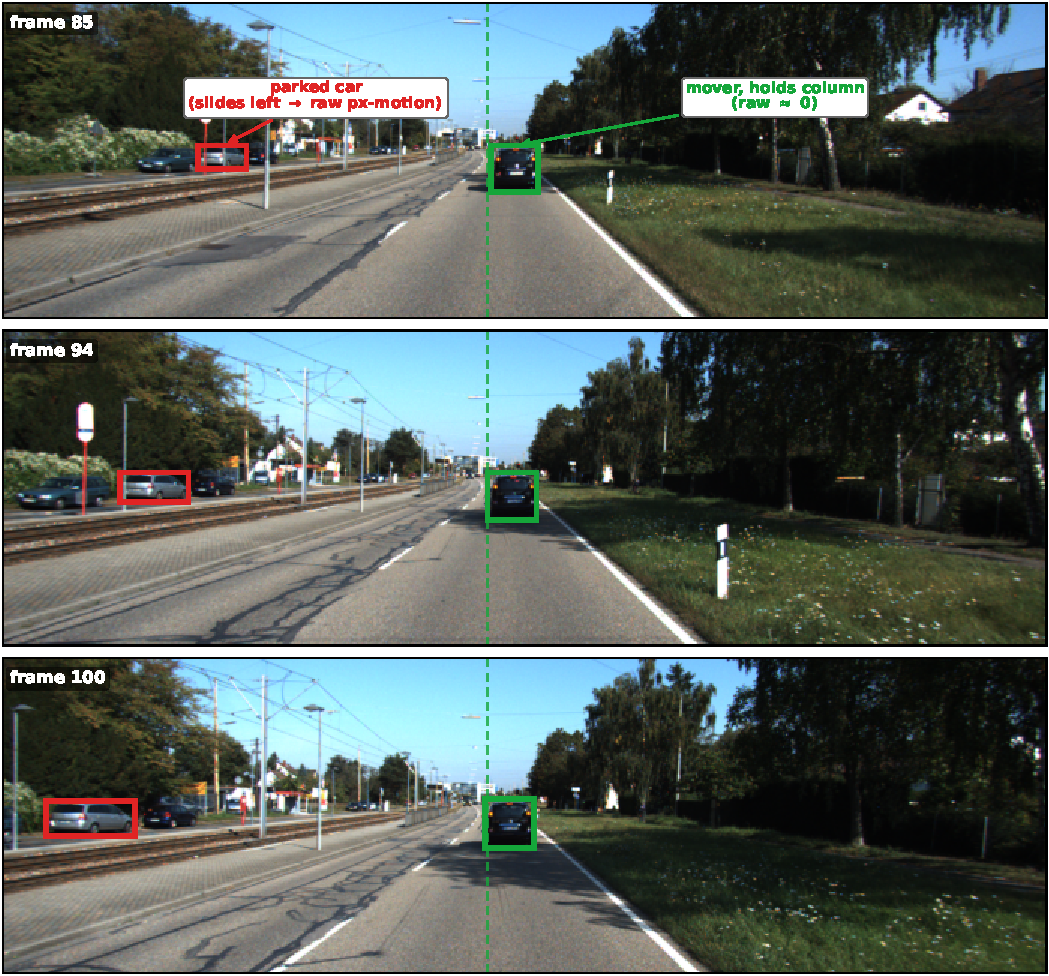
\includegraphics[width=\linewidth]{figures/qualitative.pdf}
  \caption{``Moving cars'' (Refer-KITTI seq 0005). The parked car (red) sweeps across the image as the camera passes, while the moving car (green) barely shifts. Raw image motion misclassifies both; the ego-compensated residual recovers both from the same host score.}
  \label{fig:qual}
\end{figure}

Figure~\ref{fig:qual} shows a sample tracking result. The parked car appears to move across frames due to camera motion, while the moving car remains at nearly the same distance from the camera. Without ego-motion compensation, these two cases are easily confused and mistracked. After motion compensation, the parked car has nearly zero residual velocity, while the moving car presents nonzero residual velocity. This allows the GMC module to more correctly predict the matching score.

\section{Conclusion and Limitations}
\label{sec:conclusion}
The GMC module is a plug-in that improves motion grounding in referring multi-object tracking without modifying the detector, tracker, or appearance-language matching model. By compensating for camera motion and matching residual motion features with language expressions, the proposed module helps distinguish object motion from camera-induced motion. Road-region background correspondences provide a geometric reference for estimating camera motion in driving videos. The residual motion features are then matched against language expressions to yield a matching score, which is integrated with the host model's prediction score via late fusion. On the Refer-KITTI datasets, the pooled HOTA improves for different host models. On the moving-class expressions, the largest gain is observed when iKUN is used as the host model ($+9.44\pm0.92$).

Despite these promising results, several limitations remain. First, the road-plane homography assumes a flat ground plane. Scenes with steep slopes or uneven terrain fall outside the model's scope. Second, the keyword classifier routes only moving-class expressions to $\alpha_{\mathrm{mot}}$; direction and turning expressions ($214$ of the $818$ in Refer-KITTI V1) receive the appearance weight, so the module does not help them even though they describe motion. Finally, our experiments are conducted on two RMOT frameworks and the Refer-KITTI benchmarks. Additional evaluations across more host models and datasets are needed to further validate the generality of the proposed approach.

% References should be produced using the bibtex program from suitable
% BiBTeX files (here: strings, refs, manuals). The IEEEbib.bst bibliography
% style file from IEEE produces unsorted bibliography list.
% -------------------------------------------------------------------------
\bibliographystyle{IEEEbib}
\bibliography{refs}

\end{document}
